% !TEX root = thesis.tex
\documentclass[a4paper,12pt]{report}
\usepackage{graphicx} % Required for inserting images
\usepackage[italian]{babel}
\usepackage{float}
\usepackage{longtable}
\usepackage{booktabs}
\usepackage{amsmath}
\usepackage{array}
\usepackage{subcaption}
\usepackage{url}
\usepackage[hidelinks]{hyperref}
\usepackage{biblatex}
\usepackage{csquotes}
\addbibresource{bibliografia.bib}

\title{Relazione di Tirocinio}
\author{Marco Di Giovannantonio}
\date{November 2026}

\begin{document}

\maketitle

\tableofcontents

\chapter{Introduzione}
\label{cap:introduzione}

\section{Motivazione e contesto clinico}

I reni svolgono diverse funzioni fondamentali per il corretto funzionamento dell'organismo umano: tra queste rientrano la filtrazione del sangue e l'eliminazione delle sostanze di scarto derivanti dal metabolismo, la regolazione dell'equilibrio idrico ed elettrolitico e la produzione di alcuni ormoni essenziali\cite{ogobuiro2023physiology}. Ne consegue che, quando la funzionalità renale risulta gravemente compromessa, può essere necessario ricorrere a una terapia sostitutiva, come la dialisi, per compensare almeno in parte tale perdita\cite{LOK2020S1}.

La dialisi consente di rimuovere dal sangue numerose sostanze di scarto e di contribuire alla regolazione dell'equilibrio dei liquidi e degli elettroliti, tra cui sodio, potassio, calcio e fosforo. Si tratta di una terapia fondamentale per molti pazienti affetti da insufficienza renale avanzata, il cui percorso clinico richiede un monitoraggio regolare delle condizioni di salute\cite{NANOVIC2005}.

Durante il trattamento vengono raccolte diverse tipologie di misurazioni, che possono essere distinte, sulla base della natura dei dati considerati in questo lavoro, in tre categorie:
\begin{itemize}
    \item \textbf{Valori di laboratorio}, che comprendono misurazioni effettuate periodicamente o su richiesta del medico.
    \item \textbf{Valori nutrizionali}, che comprendono misurazioni relative allo stato nutrizionale del paziente, raccolte secondo le modalità previste dal percorso clinico.
    \item \textbf{Valori dialitici}, che comprendono misurazioni associate alla singola seduta di dialisi, raccolte durante il trattamento.
\end{itemize}

Queste misurazioni, raccolte con frequenze e modalità differenti, permettono di descrivere l'evoluzione delle condizioni cliniche del paziente nel tempo. La loro osservazione longitudinale assume particolare rilevanza nei pazienti sottoposti a dialisi, per i quali l'insorgenza di complicazioni può richiedere interventi clinici specifici o il ricovero ospedaliero.

Un esempio significativo riguarda l'accesso vascolare, necessario per consentire l'esecuzione del trattamento dialitico. Esso costituisce una via di accesso al sistema circolatorio attraverso la quale il sangue viene prelevato e successivamente reimmesso nel paziente durante la terapia. Il deterioramento della sua funzionalità può rendere necessari interventi specifici e, nei casi più complessi, la predisposizione di un nuovo accesso\cite{LOK2020S1}. Poiché la gestione delle complicazioni associate all'accesso vascolare può comportare procedure invasive e costi significativi\cite{AVCCostItaly2024}, risulta importante disporre di informazioni che contribuiscano a una migliore valutazione delle condizioni cliniche del paziente.

In questo contesto, l'analisi longitudinale delle misurazioni raccolte durante il percorso dialitico rappresenta un'opportunità per studiare la relazione tra l'evoluzione delle caratteristiche cliniche del paziente e l'insorgenza di eventi avversi. Le tecniche di apprendimento automatico offrono strumenti per analizzare tali informazioni e individuare schemi nei dati potenzialmente utili a distinguere situazioni caratterizzate da una diversa distanza temporale dall'evento.

\section{Obiettivo}

Il presente lavoro si propone di valutare l'applicabilità di tecniche di apprendimento automatico alla classificazione del tempo che intercorre tra una seduta di dialisi e il primo evento avverso considerato; in particolare, ai fini del lavoro, l'endpoint è definito come il primo, in ordine cronologico, tra due eventi: il ricovero per accesso vascolare (AV) e il decesso.

A tale scopo, le misurazioni longitudinali dei pazienti vengono elaborate attraverso due differenti approcci: il primo rappresenta le misurazioni raccolte in una finestra temporale precedente alla seduta mediante il calcolo dei valori medi dei singoli parametri, mentre il secondo descrive invece il loro andamento nel tempo attraverso i coefficienti di una regressione lineare, pendenza e intercetta. L'ampiezza della finestra temporale per entrambi gli approcci è definita da un parametro espresso in giorni.

Le rappresentazioni così ottenute vengono utilizzate come input per i modelli di classificazione. Il tempo al primo evento avverso viene discretizzato in intervalli temporali definiti mediante soglie prestabilite, anziché essere stimato direttamente come una durata espressa in giorni. Il lavoro prevede pertanto una serie di esperimenti finalizzati a valutare e confrontare le rappresentazioni adottate e le prestazioni dei modelli di apprendimento automatico considerati.

L'obiettivo finale è comprendere se e in quale misura la rappresentazione delle misurazioni nel tempo possa fornire informazioni utili alla classificazione del tempo al primo evento avverso nei pazienti sottoposti a dialisi, evidenziando le potenzialità e i limiti degli approcci esaminati.

\section{Introduzione alle reti neurali LSTM}

Le reti neurali tradizionali, dette anche reti feedforward, elaborano le informazioni attraverso una successione di trasformazioni, senza mantenere uno stato interno che venga aggiornato tra i diversi elementi di una sequenza. Questa caratteristica può rappresentare un limite quando si considerano dati sequenziali, nei quali l'ordine degli elementi e le relazioni tra osservazioni successive o distanti nel tempo assumono un ruolo fondamentale. Si pensi, ad esempio, all'elaborazione del linguaggio naturale: per comprendere una frase è necessario considerare non soltanto le singole parole, ma anche il contesto fornito da quelle precedenti.

Per affrontare questo problema sono state introdotte le Reti Neurali Ricorrenti (\textit{Recurrent Neural Networks}, RNN)\cite{RNNELMAN1990179}. L'idea alla base di queste architetture consiste nell'introdurre delle connessioni ricorrenti, attraverso le quali le informazioni elaborate in un passaggio vengono trasmesse a quello successivo. In particolare, la rete mantiene uno stato interno, chiamato \textit{hidden state}, che viene aggiornato a ogni nuovo input e consente di conservare informazioni relative agli elementi precedentemente elaborati. In questo modo, la rete può processare una sequenza un elemento alla volta, tenendo conto delle informazioni acquisite nei passaggi precedenti.

Tuttavia, quando le informazioni rilevanti sono molto distanti tra loro all'interno di una sequenza, le RNN tradizionali possono incontrare difficoltà nell'apprendere le relazioni che le collegano. Una delle principali cause è il fenomeno della scomparsa del gradiente (\textit{vanishing gradient})\cite{VanishingGradient1994}, che durante l'addestramento rende sempre più difficile aggiornare i pesi della rete sulla base di informazioni provenienti da passaggi temporali lontani. In questo modo, l'influenza degli input precedenti può attenuarsi al punto da compromettere l'apprendimento delle dipendenze a lungo termine.

Per mitigare questo problema sono state introdotte le reti Long Short-Term Memory (LSTM)\cite{LSTM/neco.1997.9.8.1735}, una particolare tipologia di rete neurale ricorrente progettata per gestire meglio le dipendenze a lungo termine. Queste architetture introducono una cella di memoria (\textit{cell state}), che permette di conservare informazioni rilevanti attraverso i diversi passaggi temporali, e un sistema di porte (\textit{gates}) che regola il flusso delle informazioni. In particolare, la \textit{Forget Gate}\cite{LSTMForgetGate2000} stabilisce quali informazioni mantenere o rimuovere dalla memoria, la \textit{Input Gate} seleziona quali nuove informazioni introdurre nella cella di memoria, mentre la \textit{Output Gate} determina quali informazioni utilizzare per aggiornare lo stato nascosto. Grazie a questa struttura, le LSTM possono preservare informazioni rilevanti per intervalli temporali più ampi rispetto alle RNN tradizionali, mitigando il problema della scomparsa del gradiente.

\section{Ambito del progetto d'esame}

Il presente elaborato documenta il lavoro svolto nell'ambito del progetto di tirocinio distinguendolo dalle più contenute attività svolte per il progetto d'esame di Intelligenza Artificiale. Sebbene i due percorsi siano strettamente correlati e condividano parte del contesto applicativo e delle attività svolte, è importante precisare quali componenti siano specificamente riconducibili al progetto d'esame e quali al progetto di tirocinio.

In particolare, il progetto d'esame si concentra sulla costruzione dei dataset attraverso gli approcci basati sul calcolo delle medie e sulla stima dei coefficienti di regressione, sull'addestramento e sul confronto di modelli di apprendimento automatico, sulla gestione degli errori di inserimento e dei dati mancanti, sull'esplorazione di tecniche di ottimizzazione degli iperparametri e sulla valutazione delle prestazioni mediante tecniche di cross-validation. Comprende inoltre un'analisi di sopravvivenza attraverso l'impiego di stimatori statistici. Per questa parte del lavoro, la finestra temporale considerata (\textit{sliding window}) era fissata a 30 giorni.

Il progetto di tirocinio si pone in continuità con le attività precedenti e ne costituisce un approfondimento con l'introduzione di tecniche di ottimizzazione multi-obiettivo e lo sviluppo di ulteriori esperimenti di addestramento, finalizzati a valutare il comportamento dei modelli e le relative prestazioni rispetto alle metriche di valutazione considerate.

\section{Struttura}

Il presente elaborato è organizzato come segue: il Capitolo~\ref{cap:dataset} descrive i dati utilizzati, la loro raccolta e la costruzione del dataset; il Capitolo~\ref{cap:metodo} presenta l'approccio metodologico: la definizione delle classi di rischio, le due rappresentazioni delle misurazioni, il classificatore KNN, il classificatore LSTM, la gestione dei duplicati, la gestione degli outlier e la gestione dei missing; il Capitolo~\ref{cap:risultati} riporta gli esperimenti svolti e i risultati ottenuti.

\chapter{Dataset e preparazione dei dati}
\label{cap:dataset}
\section{Raccolta dei dati}

L'infrastruttura del DBMS e i dati contenuti nelle relative tabelle sono stati forniti dal rAIse Lab di Sapienza Università di Roma. I dati provengono da 38 emocentri distribuiti sul territorio italiano e coprono un periodo di osservazione compreso tra gennaio 2023 e giugno 2026.

Secondo le informazioni fornite dal rAIse Lab, i dati sono stati trattati nel rispetto delle disposizioni applicabili del Regolamento dell'Unione Europea (UE) 2016/679 General Data Protection Regulation (GDPR).

\section{Analisi dei dati}

I dati comprendono diverse tipologie di informazioni cliniche relative ai pazienti e alle singole sedute di dialisi. La Tabella~\ref{tab:variabili} riporta l'elenco delle variabili, specificandone l'unità di misura, l'origine e una breve descrizione. Per quanto riguarda l'origine, M indica una variabile registrata direttamente nella base di dati, mentre C identifica una variabile calcolata mediante elaborazione di altre variabili.

\providecommand{\V}[1]{\ensuremath{\text{#1}}}

\small
\renewcommand{\arraystretch}{1.2}
\begin{longtable}{@{}>{\raggedright\arraybackslash}p{3.1cm}
                   >{\raggedright\arraybackslash}p{2.4cm}
                   c
                   >{\raggedright\arraybackslash}p{7.0cm}@{}}
\caption{Variabili del dataset}
\label{tab:variabili}\\
\toprule
\textbf{Variabile} & \textbf{Unità} & \textbf{Orig.} & \textbf{Descrizione} \\
\midrule
\endfirsthead
\toprule
\textbf{Variabile} & \textbf{Unità} & \textbf{Orig.} & \textbf{Descrizione} \\
\midrule
\endhead
\midrule
\multicolumn{4}{r}{\emph{continua nella pagina successiva}} \\
\endfoot
\bottomrule
\endlastfoot

\multicolumn{4}{@{}l}{\textbf{Anagrafica e accesso vascolare}} \\
\midrule
Sesso & categorica & M & Sesso del paziente. \\
Data di nascita & data & M & Data di nascita del paziente. \\
Tipo accesso vascolare & categorica & M & Tipo di accesso vascolare: CVC permanente (CVC-Per), CVC temporaneo (CVC-Tem) o fistola arterovenosa (FAV). \\
Data installazione AV & data & M & Data di installazione dell'accesso vascolare attualmente in uso. \\
Mesi CVC & mesi & C & Mesi trascorsi tra la prima registrazione di un accesso di tipo CVC e la data della seduta. \\
Mesi FAV & mesi & C & Mesi trascorsi tra la prima registrazione di un accesso di tipo FAV e la data della seduta. \\
Score CVC & intero & M & Punteggio di valutazione dell'accesso vascolare di tipo CVC. \\
Score FAV & intero & M & Punteggio di valutazione dell'accesso vascolare di tipo FAV. \\
Score coag & intero & M & Punteggio relativo alla presenza di coaguli. \\
\midrule

\multicolumn{4}{@{}l}{\textbf{Variabili dialitiche (per seduta)}} \\
\midrule
Minuti dialisi & min & C & Durata della seduta di dialisi, calcolata a partire dall'intervallo dell'evento. \\
Ore dialisi & h & C & $\V{Minuti dialisi}/60$. \\
Peso pre & kg & M & Peso del paziente prima della seduta. \\
Peso post & kg & M & Peso del paziente dopo la seduta. \\
UF tot & kg & C & Differenza tra peso pre e peso post, utilizzata come stima dell'ultrafiltrazione netta: $\V{Peso pre} - \V{Peso post}$. \\
UF & mL/(h$\cdot$kg) & C & Tasso di ultrafiltrazione normalizzato: $\V{UF tot}/(\V{Ore dialisi}\cdot\V{Peso post})\cdot 1000$. \\
QB totale & L & M & Volume totale di sangue trattato durante la seduta. \\
QB medio & mL/min & M & Flusso ematico medio durante la seduta. \\
QB & mL/min & C & Flusso ematico medio calcolato a partire dal volume totale di sangue trattato e dalla durata della seduta: $\V{QB totale}/\V{Minuti dialisi}\cdot 1000$. \\
Arter & mmHg & M & Pressione dinamica arteriosa. \\
Vena & mmHg & M & Pressione dinamica venosa. \\
A/V & --- & C & Rapporto tra pressione arteriosa e pressione venosa: $\V{Arter}/\V{Vena}$. \\
PA/QB & mmHg\slash(mL/min) & C & Pressione arteriosa normalizzata per il flusso ematico: $\V{Arter}/\V{QB}$. \\
PV/QB & mmHg\slash(mL/min) & C & Pressione venosa normalizzata per il flusso ematico: $\V{Vena}/\V{QB}$. \\
Azotemia pre & mg/dL & M & Azoto ureico (BUN) prima della seduta. \\
Azotemia post & mg/dL & M & Azoto ureico (BUN) dopo la seduta. \\
\midrule

\multicolumn{4}{@{}l}{\textbf{Valori nutrizionali}} \\
\midrule
BMI & kg/m$^2$ & M & Indice di massa corporea. \\
Circonferenza braccio & cm & M & Circonferenza del braccio. \\
DPI & g/giorno & M & Apporto proteico alimentare (\emph{dietary protein intake}). \\
DEI & kcal/giorno & M & Apporto energetico alimentare (\emph{dietary energy intake}). \\
DPI/Peso & g/(giorno$\cdot$kg) & C & Rapporto tra apporto proteico alimentare e peso post: $\V{DPI}/\V{Peso post}$. \\
DEI/Peso & kcal\slash(giorno$\cdot$kg) & C & Rapporto tra apporto energetico alimentare e peso post: $\V{DEI}/\V{Peso post}$. \\
FFM post & kg & M & Massa priva di grasso, misurata dopo la seduta. \\
BCM post & kg & M & Massa cellulare corporea, misurata dopo la seduta. \\
FM post & kg & M & Massa grassa, misurata dopo la seduta. \\
Albuminemia & g/dL & M & Concentrazione sierica di albumina. \\
Colesterolemia & mg/dL & M & Concentrazione sierica di colesterolo. \\
\midrule

\multicolumn{4}{@{}l}{\textbf{Valori di laboratorio e terapia}} \\
\midrule
Hb & g/dL & M & Emoglobina. \\
Sideremia & $\mu$g/dL & M & Concentrazione sierica di ferro. \\
Transferrina & mg/dL & M & Concentrazione sierica di transferrina. \\
Ferritina & ng/mL & M & Concentrazione sierica di ferritina. \\
TSAT & \% & C & Saturazione della transferrina: $\V{Sideremia}/(\V{Transferrina}\cdot 1.42)\cdot 100$. \\
Dosaggio epoetina alpha mensile & UI & M & Dose mensile di epoetina alfa. \\
Alpha EPODose Weight & UI/(kg$\cdot$sett.) & C & Dose settimanale di epoetina per kg: $(\V{Dosaggio epoetina alpha mensile}/30\cdot 7)/\V{Peso post}$. \\
Alpha ERI & UI\slash(kg$\cdot$sett.)\slash(g/dL) & C & Indice di resistenza all'eritropoietina: $\V{Alpha EPODose Weight}/\V{Hb}$. \\
Calcemia & mg/dL & M & Concentrazione sierica di calcio. \\
Fosforemia & mg/dL & M & Concentrazione sierica di fosforo. \\
PTH & pg/mL & M & Concentrazione del paratormone. \\
Fosfatasi alcalina & UI/L & M & Attività sierica della fosfatasi alcalina. \\
FosfAlcIndex & --- & C & Fosfatasi alcalina normalizzata a 120 UI/L: $\V{Fosfatasi alcalina}/120$. \\
Vitamina D & ng/mL & M & Concentrazione di vitamina D. \\
Bicarbonatemia & mEq/L & M & Concentrazione sierica di bicarbonato. \\
\end{longtable}
\normalsize

I dati sono stati organizzati in varie tabelle relazionali; vengono introdotte quelle utilizzate maggiormente in questo elaborato: 
\begin{itemize}
    \item Patient.PropertyMeasure, tabella che contiene tutte le misurazioni, l'identificativo del paziente a cui si riferiscono e l'identificativo dell'evento a cui si riferiscono; quest'ultimo può essere vuoto.
    \item Patient.PatientEvent, tabella che contiene tutti gli eventi e l'identificativo del paziente a cui si riferisce; di questa tabella fanno parte i ricoveri per accesso vascolare, i decessi, i ricoveri per altro, e le sedute di dialisi.
\end{itemize}

Per dare una visione d'insieme al lettore e consentirgli di familiarizzare con i dati, per quanto possibile, vengono riportati i seguenti dati macroscopici:
\begin{itemize}
    \item Pazienti totali: 3205.
    \item Pazienti distinti con decesso: 851.
    \item Pazienti distinti con ricovero per accesso vascolare: 1941.
    \item Pazienti distinti con almeno una seduta di dialisi: 2952.
    \item Pazienti distinti con evento avverso dopo l'inizio della storia dialitica: 1201.
\end{itemize}

È opportuno chiarire la discrepanza tra i pazienti distinti con ricovero per accesso vascolare (1941) e i pazienti distinti con evento avverso dopo l'inizio della storia dialitica (1201): tale discrepanza potrebbe essere spiegata dall'ipotesi che, per alcuni pazienti, il primo ricovero per accesso vascolare sia finalizzato alla predisposizione dell'accesso stesso e preceda l'inizio effettivo del trattamento dialitico. Di conseguenza, ai fini della presente analisi, l'inizio della storia clinica del paziente viene fatta coincidere con la prima seduta dialitica, mentre viene considerato come primo evento avverso quello eventualmente verificatosi successivamente a tale data.

La Figura \ref{fig:dialysis_sess_boxplot} mostra la distribuzione del numero di sedute di dialisi per paziente per i pazienti nella popolazione considerata.

\begin{figure}[H]
    \centering
    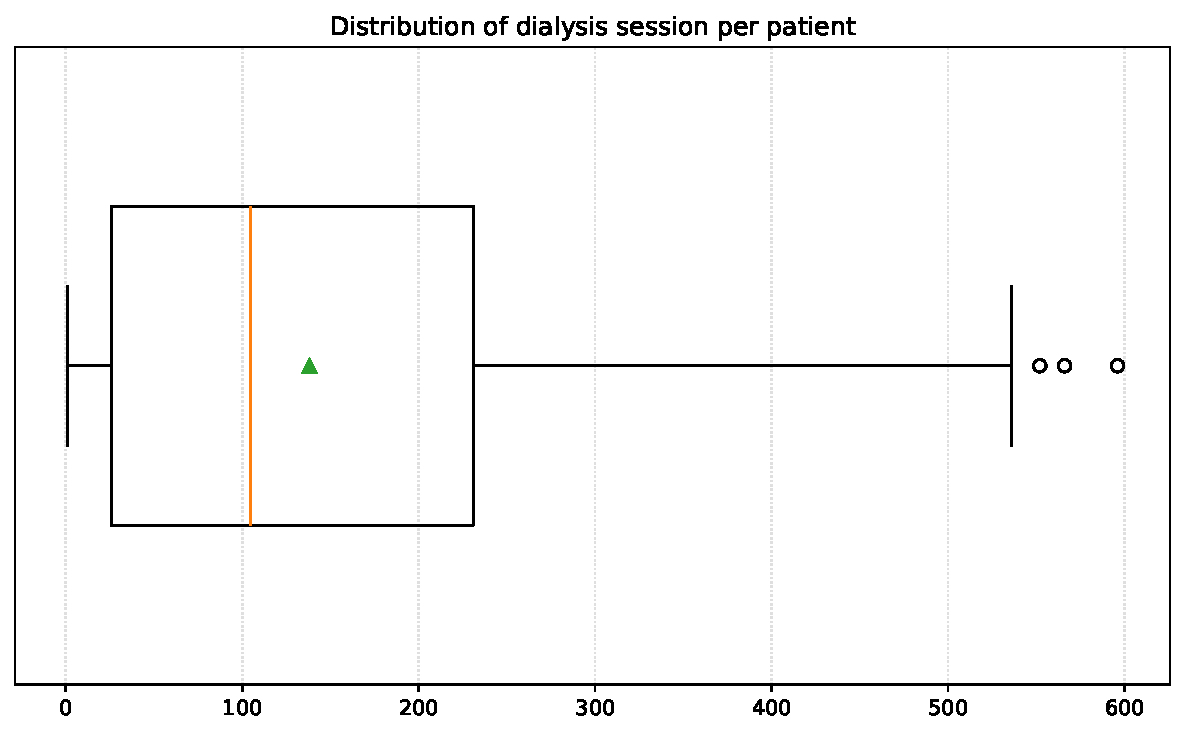
\includegraphics[width=1\linewidth]{dialysis_session_boxplot.pdf}
    \caption{Distribuzione del numero di sedute di dialisi per paziente}
    \label{fig:dialysis_sess_boxplot}
\end{figure}

La Tabella \ref{tab:intervalli_dialisi} mostra le distribuzioni degli intervalli in giorni che intercorrono tra sedute consecutive di dialisi di uno stesso paziente.

\begin{table}[H]
\centering
\caption{Distribuzione degli intervalli in giorni tra sedute consecutive di dialisi}
\label{tab:intervalli_dialisi}

\begin{tabular}{|l|c|}
\hline
\textbf{Statistica} & \textbf{Intervallo (giorni)} \\
\hline
$5^{\circ}$ percentile & 1,799 \\
$10^{\circ}$ percentile & 1,986 \\
$25^{\circ}$ percentile & 2,000 \\
Mediana & 2,000 \\
$75^{\circ}$ percentile & 3,000 \\
$90^{\circ}$ percentile & 3,003 \\
\hline
\end{tabular}
\end{table}

I valori riportati mostrano che la mediana dell'intervallo tra due sedute consecutive è pari a 2 giorni. Si osserva tuttavia una certa variabilità, evidenziata dalla differenza tra il 25$^\circ$ e il 75$^\circ$ percentile, che assume rispettivamente valori pari a 2 e 3 giorni

La Tabella \ref{tab:percentili_proprieta} mostra la distribuzione dei tempi che intercorrono tra una misurazione di laboratorio o nutrizionale e la seduta di dialisi successiva più vicina nel tempo.

\begin{table}[H]
\centering
\caption{Distribuzione dei tempi tra misurazione e seduta di dialisi successiva, per proprietà}
\label{tab:percentili_proprieta}
\scriptsize
\setlength{\tabcolsep}{3pt}
\renewcommand{\arraystretch}{1.05}

\resizebox{\linewidth}{!}{%
\begin{tabular}{lrrrrrrr}
\hline
\textbf{Proprietà} &
\textbf{P25} &
\textbf{P50} &
\textbf{P75} &
\textbf{P80} &
\textbf{P85} &
\textbf{P90} &
\textbf{P95} \\
\hline
Albuminemia & 0,292 & 0,521 & 1,708 & 1,757 & 5,500 & 74,750 & 146,562 \\
Azotemia Post & 0,292 & 0,521 & 1,708 & 1,792 & 4,505 & 64,640 & 154,500 \\
Azotemia Pre & 0,292 & 0,507 & 1,698 & 1,753 & 6,708 & 65,271 & 154,271 \\
BCM post & 1,784 & 1,882 & 2,854 & 2,893 & 3,821 & 62,866 & 221,776 \\
Bicarbonatemia & 0,292 & 0,500 & 0,708 & 0,750 & 0,792 & 1,708 & 1,740 \\
Calcemia & 0,294 & 0,542 & 1,792 & 1,977 & 8,500 & 65,981 & 156,259 \\
Circonferenza Braccio & 0,292 & 0,500 & 0,708 & 0,757 & 1,281 & 1,490 & 1,708 \\
Colesterolemia & 0,294 & 0,542 & 1,750 & 2,016 & 8,837 & 77,278 & 168,561 \\
DEI & 0,313 & 0,552 & 1,479 & 1,500 & 1,542 & 1,719 & 2,542 \\
DPI & 0,313 & 0,552 & 1,479 & 1,500 & 1,542 & 1,715 & 2,542 \\
Dosaggio Epoetina Alpha mensile & 0,500 & 1,292 & 1,701 & 2,271 & 2,314 & 2,524 & 3,292 \\
FFM post & 1,784 & 1,882 & 2,854 & 2,893 & 3,821 & 62,866 & 221,776 \\
FM post & 1,784 & 1,882 & 2,854 & 2,893 & 3,822 & 62,866 & 221,776 \\
Ferritina & 0,292 & 0,524 & 1,708 & 1,792 & 9,442 & 65,271 & 154,501 \\
Fosfatasi Alcalina & 0,292 & 0,514 & 1,698 & 1,750 & 3,271 & 49,232 & 115,647 \\
Fosforemia & 0,299 & 0,552 & 1,864 & 3,320 & 37,292 & 91,271 & 182,271 \\
Hb & 0,297 & 0,542 & 1,792 & 1,981 & 4,500 & 58,750 & 152,914 \\
PTH & 0,292 & 0,524 & 1,708 & 1,792 & 10,441 & 70,492 & 161,667 \\
Sideremia & 0,299 & 0,542 & 1,792 & 2,022 & 4,492 & 57,660 & 154,543 \\
Transferrina & 0,292 & 0,528 & 1,708 & 1,792 & 11,708 & 65,971 & 156,289 \\
Vitamina D & 0,295 & 0,542 & 1,771 & 11,458 & 75,098 & 92,708 & 182,500 \\
\hline
\end{tabular}%
}
\vspace{2mm}

\footnotesize
\textit{Nota:} P25--P95 indicano rispettivamente il 25$^{\circ}$--95$^{\circ}$ percentile.
I valori sono espressi in giorni.
\end{table}

I valori riportati evidenziano una notevole variabilità nella frequenza di raccolta delle diverse misurazioni. Alcune proprietà presentano osservazioni frequentemente disponibili a breve distanza dalle sedute di dialisi, mentre altre sono caratterizzate da intervalli temporali considerevolmente più ampi. Questa eterogeneità rende necessario adottare criteri specifici per ciascuna proprietà nella successiva associazione delle misurazioni alle sedute.

\section{Produzione del dataset}

A partire dalle tabelle del DBMS, è stato costruito un dataset che associa a ciascuna seduta di dialisi le misurazioni disponibili per il relativo paziente. Poiché le diverse tipologie di misurazioni non sono necessariamente collegate direttamente a un evento di dialisi, sono state adottate modalità differenti per associarle alla seduta.

In particolare, è stato utilizzato il seguente approccio:

\begin{itemize}
    \item Le misurazioni relative ad un evento di dialisi sono state aggregate insieme attraverso la relazione con l'id dell'evento di dialisi.
    \item Le misurazioni di laboratorio e nutrizionali, non essendo direttamente associate agli eventi di dialisi, sono state collegate alle sedute sulla base della loro vicinanza temporale. Per ciascuna proprietà è stata definita una soglia massima di anzianità, indicata con \(age_m\), oltre la quale la misurazione non viene considerata.
    \item Per le variabili che non cambiano o che cambiano raramente nel tempo, come il tipo di accesso vascolare, è stato recuperato l'ultimo valore osservato alla data della seduta di dialisi.
\end{itemize}

I pazienti che non hanno avuto un evento avverso nel periodo di osservazione vengono ugualmente considerati ai fini dell'analisi di sopravvivenza, in quanto forniscono informazioni utili: non verranno dunque esclusi dal dataset.

La definizione dei criteri temporali per l'associazione delle misurazioni è stata preceduta da un'analisi delle distanze temporali tra le sedute di dialisi e tra le misurazioni e le relative sedute. In primo luogo, è stata analizzata la distribuzione degli intervalli tra sedute consecutive dello stesso paziente, riportata nella Tabella~\ref{tab:intervalli_dialisi}. Questa analisi consente di caratterizzare la frequenza delle sedute e di individuare gli intervalli temporali più comuni tra due trattamenti consecutivi. Successivamente, è stata studiata la distanza temporale tra ciascuna misurazione e la seduta di dialisi a cui potrebbe essere associata. La Tabella~\ref{tab:percentili_proprieta} riporta, per ogni proprietà, alcuni percentili della distribuzione di tali distanze, espressi in giorni. Questi valori permettono di valutare la disponibilità delle misurazioni e la loro effettiva vicinanza temporale alle sedute di dialisi.

Sulla base di queste analisi sono stati definiti i parametri \(age_m\), specifici per ciascuna proprietà, utilizzati per stabilire l'intervallo temporale massimo entro cui una misurazione può essere associata a una seduta. In particolare, ai fini del lavoro, è stata impostata come soglia massima il 10$^{\circ}$ percentile degli intervalli tra sedute di dialisi: di ogni proprietà è stato scelto il percentile che più si avvicinava a esso ed è stato applicato un arrotondamento per eccesso alla prima o seconda cifra decimale; per le proprietà con il 75$^{\circ}$ percentile più alto della soglia massima, è stata presa la soglia massima. Tale analisi è necessaria perché limita il bias statistico introdotto dal \textit{Last Observation Carried Forward} (LOCF).

Il dataset risultante è organizzato a livello di seduta: ciascuna riga identifica un paziente, la data della seduta di dialisi e l'insieme delle misurazioni associate secondo i criteri descritti; le righe sono ordinate per paziente e per data di dialisi.

A ciascuna seduta di dialisi è inoltre associata una variabile temporale derivata, denominata \textit{Time To Event} (TTE), che rappresenta la distanza in giorni tra la data della seduta e quella del primo evento avverso successivo nella storia clinica del paziente. Gli eventi avversi considerati comprendono il ricovero per accesso vascolare e il decesso. Questa variabile consente di descrivere il tempo che intercorre tra la seduta di dialisi e l'eventuale comparsa di un evento avverso.

Per l'analisi viene fissato un orizzonte di predizione (\textit{prediction horizon}), indicato con \(H\), pari a 400 giorni. Tale scelta consente di limitare la previsione degli eventi avversi a un intervallo temporale definito, considerando come rilevanti gli eventi che si verificano strettamente entro tale periodo. Viene pertanto definita la variabile \(TTE_H\), ottenuta limitando il valore del TTE all'orizzonte considerato:

\[
TTE_H = \min(TTE, H)
\]

In questo modo, tutti i TTE superiori all'orizzonte di predizione vengono ricondotti a 400 giorni. Lo stesso valore viene assegnato alle osservazioni per le quali non viene rilevato alcun evento entro tale intervallo, purché sia disponibile un periodo di osservazione sufficiente a verificarne l'assenza.

A ciascuna seduta viene quindi associata anche una variabile binaria, denominata \texttt{event\_observed}, che indica se l'evento avverso si è verificato prima del termine dell'orizzonte di predizione. La variabile è definita come:

\[
\texttt{event\_observed} =
\begin{cases}
1 & \text{se } TTE_H < H\\
0 & \text{altrimenti}
\end{cases}
\]

Pertanto, un valore pari a 1 identifica le osservazioni caratterizzate dalla presenza di un evento avverso strettamente entro l'orizzonte temporale, mentre un valori pari a 0 identifica quelle per le quali non viene osservato alcun evento avverso entro tale intervallo.

Le osservazioni relative ai pazienti per i quali non viene registrato alcun evento avverso non vengono escluse a priori, poiché forniscono informazioni utili per l'analisi. Tuttavia, per assegnare correttamente il valore 0 alla variabile \texttt{event\_observed}, è necessario disporre di un periodo di osservazione di almeno 400 giorni successivi alla seduta di dialisi. Per questo motivo, vengono escluse le singole osservazioni relative ai pazienti senza evento avverso per le quali il follow-up disponibile risulta inferiore a tale intervallo.

\chapter{Approccio metodologico}
\label{cap:metodo}
\section{Specifiche Tecniche}

Il presente lavoro di tesi adotta un'impostazione di tipo \textit{dynamic landmark}, nel quale ciascuna seduta di dialisi costituisce un nuovo punto di riferimento temporale rispetto al quale viene aggiornata la previsione; tale riferimento temporale è dunque sia un \textit{landmark time} sia un \textit{prediction time} \cite{VANHOUWELINGENDL2006}. Vengono inoltre utilizzati due approcci diversi per la gestione e la classificazione del rischio.

Sia \(D\) il dataset, composto da righe della forma:
\[
r_{p,d} = (d,p,m_1,\ldots,m_n)
\]
dove \(d\) rappresenta la data della seduta di dialisi, \(p\) l'identificativo del paziente e \(m_1,\ldots,m_n\) i valori delle variabili associate alla relativa seduta. La coppia \((d,p)\) identifica univocamente ciascuna riga del dataset.

Sia \(F\) l'insieme delle feature considerate e sia \(w\) l'ampiezza, espressa in giorni, della finestra temporale.

Per ogni paziente \(p\), data di riferimento \(d\) e feature \(f\in F\), vengono considerate le osservazioni appartenenti alla finestra temporale \([d-w,d]\), estremi inclusi. Si definisce pertanto:
\[
\mathcal{M}_{p,d,f}^{(w)} =
\left\{
(t,m_{p,t,f}) \mid
d-w\leq t\leq d
\right\}
\]
dove \(m_{p,t,f}\) rappresenta il valore della feature \(f\), misurato sul paziente \(p\) alla data \(t\).

Ai fini dei calcoli successivi, vengono considerate esclusivamente le osservazioni caratterizzate da un valore disponibile. Si definisce quindi il sottoinsieme:
\[
\mathcal{M}_{p,d,f}^{*(w)} =
\left\{
(t,m_{p,t,f})\in\mathcal{M}_{p,d,f}^{(w)}
\mid m_{p,t,f}\neq\mathrm{NA}
\right\}
\]
A partire dal dataset originale vengono costruite due rappresentazioni alternative delle misurazioni, attraverso due differenti approcci statistici.

Nel primo approccio, per ogni riga del dataset originale e per ciascuna feature numerica considerata, viene calcolata la media aritmetica dei valori disponibili nella finestra temporale di riferimento.

La media viene definita come:
\[
\overline{m}_{p,d,f}^{(w)} =
\begin{cases}
\displaystyle
\frac{1}{|\mathcal{M}_{p,d,f}^{*(w)}|}
\sum_{(t,m_{p,t,f})\in\mathcal{M}_{p,d,f}^{*(w)}}
m_{p,t,f}
& \text{se }
|\mathcal{M}_{p,d,f}^{*(w)}|\geq 1 \\[12pt]
\mathrm{NA}
& \text{se }
|\mathcal{M}_{p,d,f}^{*(w)}|=0
\end{cases}
\]

La condizione \(|\mathcal{M}_{p,d,f}^{*(w)}|\geq 1\) stabilisce che è sufficiente almeno un'osservazione disponibile affinché venga calcolata la media. In assenza di osservazioni disponibili, il valore risultante viene considerato mancante.

Il dataset ottenuto, denominato dataset A, mantiene la struttura identificativa del dataset, sostituendo ciascuna feature numerica considerata con la media dei valori osservati nella relativa finestra temporale. Le feature non sottoposte ad aggregazione, come quelle categoriche e le informazioni anagrafiche, vengono invece mantenute nella loro rappresentazione originale.

Indicando con \(F_{\mathrm{agg}}\) l'insieme delle feature sottoposte al calcolo della media e con \(F_{\mathrm{keep}}\) l'insieme delle feature mantenute inalterate, il dataset A può essere formalizzato come:

\[
D_A =
\left\{
r^A_{p,d}\mid r_{p,d}\in D
\right\}
\]

dove ciascuna riga è definita come:

\[
r^A_{p,d} =
\left(
d,p,
\left(\overline{m}_{p,d,f}^{(w)}\right)_{f\in F_{\mathrm{agg}}},
\left(m_{p,d,g}\right)_{g\in F_{\mathrm{keep}}}
\right)
\]

Nel secondo approccio, per ogni riga del dataset originale e per ciascuna feature numerica considerata, viene stimata una regressione lineare sui valori osservati nella finestra temporale di riferimento.

Per stimare la regressione lineare vengono definiti:
\[
\overline{t}_{p,d,f}^{(w)}
=
\frac{1}{\left|\mathcal{M}_{p,d,f}^{*(w)}\right|}
\sum_{(t,m)\in\mathcal{M}_{p,d,f}^{*(w)}}
(t-d)
\]

\[
\overline{Y}_{p,d,f}^{(w)}
=
\frac{1}{\left|\mathcal{M}_{p,d,f}^{*(w)}\right|}
\sum_{(t,m)\in\mathcal{M}_{p,d,f}^{*(w)}}
m
\]

\[
\hat{\beta}_{1,p,d,f}^{(w)}
=
\frac{
\displaystyle
\sum_{(t,m)\in\mathcal{M}_{p,d,f}^{*(w)}}
\left[(t-d)-\overline{t}_{p,d,f}^{(w)}\right]
\left[m-\overline{Y}_{p,d,f}^{(w)}\right]
}{
\displaystyle
\sum_{(t,m)\in\mathcal{M}_{p,d,f}^{*(w)}}
\left[(t-d)-\overline{t}_{p,d,f}^{(w)}\right]^2
}
\]

\[
\hat{\beta}_{0,p,d,f}^{(w)}
=
\overline{Y}_{p,d,f}^{(w)}
-
\hat{\beta}_{1,p,d,f}^{(w)}
\overline{t}_{p,d,f}^{(w)}
\]

Dove \(\overline{t}_{p,d,f}^{(w)}\) indica la media degli scarti temporali \(t-d\), espressi in giorni, relativi alle osservazioni della feature \(f\) appartenenti all'insieme \(\mathcal{M}_{p,d,f}^{*(w)}\); \(\overline{Y}_{p,d,f}^{(w)}\) indica la media dei corrispondenti valori osservati della feature \(f\), per il paziente \(p\), nella finestra temporale \([d-w,d]\). I coefficienti \(\hat{\beta}_{1,p,d,f}^{(w)}\) e \(\hat{\beta}_{0,p,d,f}^{(w)}\) rappresentano, rispettivamente, la pendenza e l'intercetta stimate della retta di regressione.

Il dataset ottenuto, denominato dataset B, mantiene le colonne originali e aggiunge, per ciascuna feature numerica considerata, i coefficienti della regressione lineare stimati nella relativa finestra temporale.

Il dataset B può essere formalizzato come:

\[
D_B =
\left\{
r^B_{p,d}\mid r_{p,d}\in D
\right\}
\]

dove ciascuna riga è definita come:

\[
r^B_{p,d} =
\left(
d,p,
\left(m_{p,d,f}\right)_{f\in F_{\mathrm{agg}}},
\left(
\hat{\beta}_{0,p,d,f}^{(w)},
\hat{\beta}_{1,p,d,f}^{(w)}
\right)_{f\in F_{\mathrm{agg}}},
\left(m_{p,d,g}\right)_{g\in F_{\mathrm{keep}}}
\right)
\]

% Sia \(w\) l'ampiezza, espressa in giorni, della finestra temporale considerata e sia \(d\) la data della seduta di dialisi di riferimento. Per ogni paziente e per ciascuna variabile clinica, vengono considerate le misurazioni disponibili nell'intervallo temporale \([d-w,d]\), estremi inclusi. La coppia formata dall'id dell'evento di dialisi e dall'id del paziente identificano univocamente un insieme di misurazioni effettuato alla data \(d\).

% A partire dal dataset originale vengono costruite due rappresentazioni alternative delle misurazioni, attraverso due approcci differenti. Per entrambe le rappresentazioni, la sliding window è fissata a 30 giorni (non più vero, adesso ho sliding window di 30, 60, 90, 120, 150, 180 giorni, ma fa parte degli esperimenti quindi non va detto in questo capitolo.).

% Nel primo approccio, per ogni riga del dataset originale e per ciascuna variabile clinica considerata, viene calcolata la media dei valori osservati nella finestra temporale di riferimento. In questo modo, ogni riga del nuovo dataset contiene, per ciascuna variabile, il valore medio delle misurazioni disponibili nell'intervallo considerato. Il dataset ottenuto viene denominato dataset A.

% Nel secondo approccio, per ogni riga del dataset originale e per ciascuna variabile clinica considerata, viene stimata una regressione lineare sui valori osservati nella stessa finestra temporale. Per ogni variabile vengono estratti i coefficienti della retta stimata, ovvero la pendenza e l'intercetta, che descrivono rispettivamente l'andamento della variabile nel tempo e il valore previsto dalla retta in corrispondenza dell'origine temporale scelta. Il dataset ottenuto viene denominato dataset B.

% Alcune variabili non vengono sottoposte al calcolo della media o alla regressione lineare, in quanto non adatte a queste operazioni. Tra queste rientrano le variabili categoriche, come il sesso e il tipo di accesso vascolare, e le informazioni anagrafiche, come la data di nascita, e l'anzianità dell'accesso vascolare. Tali variabili non vengono tuttavia rimosse dai dataset.

A ciascuna riga dei dataset A e B viene associata una classe target, definita sulla base del tempo che intercorre tra la data della seduta di riferimento e l'evento avverso, espresso in giorni e indicato con \(TTE\). Vengono definite tre classi:

\begin{itemize}
    \item \textbf{Rosso (\(0\))}: evento avverso con \(0 \leq TTE < 180\) giorni;
    \item \textbf{Giallo (\(1\))}: evento avverso con \(180 \leq TTE < 365\) giorni;
    \item \textbf{Verde (\(2\))}: evento avverso con \(TTE \geq 365\) giorni.
\end{itemize}

La Figura \ref{fig:distribution_target_class} mostra la distribuzione delle classi di rischio.

\begin{figure}[H]
    \centering
    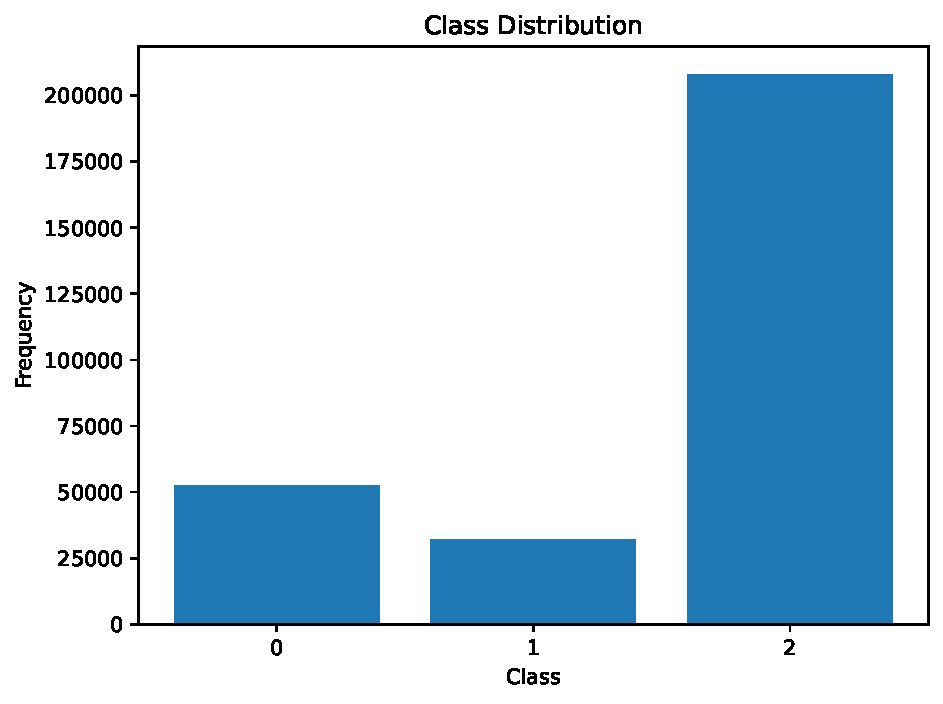
\includegraphics[width=1\linewidth]{class_distribution.pdf}
    \caption{Distribuzione delle classi di rischio}
    \label{fig:distribution_target_class}
\end{figure}

Come si evince dalla Figura \ref{fig:distribution_target_class}, le classi di rischio sono molto sbilanciate a favore della classe 2, quella a basso rischio.

\section{Gestione degli outlier}

All'interno del dataset sono stati individuati alcuni errori di inserimento. È importante precisare che tali valori possono essere valori statisticamente inconsueti, oppure errori di inserimento. Gli errori di inserimento possono essere classificati in due modi:

\begin{itemize}
    \item Errori di inserimento fuori scala, ovvero inserimento di valori clinicamente impossibili. Ad esempio, una persona non può avere un BMI negativo.
    \item Errori di inserimento nella time-series, ovvero inserimento di valori che, pur potendo essere plausibili se considerati singolarmente, risultano anomali rispetto alle misurazioni precedenti del paziente. Ad esempio, un paziente che ha avuto spesso un BMI che oscilla tra 20 e 21 potrebbe presentare un valore pari a 40 in una seduta e tornare a 21 nella seduta successiva.
\end{itemize}

In questo contesto, si definiscono \textit{outlier} le osservazioni che presentano uno scostamento significativo rispetto ai valori o alle combinazioni di valori attesi. La presenza di un outlier non implica necessariamente che il dato sia errato, ma individua un'osservazione potenzialmente anomala che potrebbe derivare da un errore di inserimento.

Per individuare tali osservazioni viene utilizzato Isolation Forest \cite{IF4781136}, un algoritmo di apprendimento non supervisionato per l'\textit{anomaly
detection}. L'algoritmo si basa sul principio secondo cui le osservazioni anomale tendono a essere più facilmente isolabili rispetto alle osservazioni ordinarie.

Isolation Forest utilizza un insieme di alberi decisionali casuali, chiamati Isolation Tree. Ogni albero viene costruito attraverso una serie di suddivisioni casuali dei dati. A ogni passaggio viene selezionata casualmente una variabile e una soglia di separazione, compresa tra il valore minimo e quello massimo osservato per la variabile selezionata, in modo da dividere le osservazioni in due gruppi. Il procedimento viene ripetuto fino a quando le osservazioni vengono isolate\cite{IF4781136}.

Il principio alla base dell'algoritmo è che un valore anomalo, essendo generalmente meno frequente e più distante dagli altri valori, tende a essere isolato attraverso un numero inferiore di suddivisioni. Per ogni osservazione viene quindi considerato il numero di passaggi necessari per isolarla nei diversi alberi. Questo valore, chiamato path length, viene utilizzato per calcolare un punteggio di anomalia (anomaly score). Valori con un percorso medio più breve tendono a essere considerati più anomali rispetto agli altri\cite{10.1145/2133360.2133363}.

Nel corso degli anni, tale algoritmo è riuscito a classificarsi come un algoritmo dall'ottima precisione nelle time-series \cite{DOMINGUES2018406} ed anche in ambito medico \cite{AnomalyDetectionEHR2023}.

Nel lavoro vengono utilizzati 1000 alberi per la costruzione dell'ensemble, impostando il parametro \(n\_estimators=1000\). Per determinare la soglia utilizzata nella classificazione delle osservazioni viene inoltre impostato il parametro \(contamination=0.0001\), corrispondente a una proporzione attesa di anomalie pari allo 0,01\% delle osservazioni analizzate. Questo parametro influenza quindi la soglia a partire dalla quale un'osservazione viene classificata come anomala, senza rappresentare un limite numerico specifico della variabile clinica.

Nel contesto considerato, Isolation Forest viene applicato globalmente, considerando tutte le osservazioni disponibili per ciascuna variabile, senza costruire un modello specifico per ogni paziente. Inoltre, le variabili vengono analizzate singolarmente, senza considerare contemporaneamente le altre misurazioni cliniche. L'algoritmo valuta quindi quanto un valore sia anomalo rispetto alla distribuzione complessiva della variabile analizzata.

È importante precisare che, anche se i dati sono organizzati in serie temporali, l'implementazione utilizzata non considera direttamente la successione delle misurazioni e non confronta ogni valore con la storia precedente del singolo paziente. Di conseguenza, un valore anomalo rispetto alla storia individuale del paziente potrebbe non essere individuato se risulta comunque compatibile con la distribuzione complessiva della variabile.

Le osservazioni identificate come anomale vengono eliminate dal dataset utilizzato per le successive analisi. In questo modo si cerca di ridurre l'influenza degli errori di inserimento e dei valori estremi sui risultati delle elaborazioni successive.

È importante sottolineare che un valore identificato come anomalo dall'algoritmo non rappresenta necessariamente un errore clinico: Isolation Forest individua valori statisticamente inconsueti, ma non dispone di conoscenze cliniche per stabilire se una misurazione sia effettivamente impossibile o errata. La classificazione ottenuta deve quindi essere interpretata come un'indicazione statistica e non come una validazione clinica del dato.

\section{Gestione dei missing}

A seguito delle politiche di aggregazione e a causa della natura dei dati, le righe presentano dei valori mancanti. I valori mancanti vengono descritti dalla Tabella \ref{tab:missing_plain}.

\begin{longtable}{p{0.72\textwidth}r}
\caption{Percentuale di valori mancanti per variabile nel dataset \textit{plain}}
\label{tab:missing_plain} \\
\toprule
\textbf{Variabile} & \textbf{Valori mancanti (\%)} \\
\midrule
\endfirsthead

\multicolumn{2}{c}{\tablename\ \thetable{} continua dalla pagina precedente} \\
\toprule
\textbf{Variabile} & \textbf{Valori mancanti (\%)} \\
\midrule
\endhead

\midrule
\multicolumn{2}{r}{Continua nella pagina successiva} \\
\endfoot

\bottomrule
\endlastfoot

\texttt{patient} & 0,00 \\
\texttt{dialysis\_date} & 0,00 \\
\texttt{dialysis\_end} & 0,00 \\
\texttt{tte\_days} & 0,00 \\
\texttt{event\_observed} & 0,00 \\
\texttt{bmi} & 12,76 \\
\texttt{score\_coag} & 100,00 \\
\texttt{qb\_totale} & 4,77 \\
\texttt{qb\_medio} & 0,02 \\
\texttt{arter} & 9,56 \\
\texttt{vena} & 10,07 \\
\texttt{score\_fav} & 96,27 \\
\texttt{score\_cvc} & 97,82 \\
\texttt{peso\_pre} & 0,10 \\
\texttt{peso\_post} & 0,19 \\
\texttt{circonferenza\_braccio} & 99,29 \\
\texttt{dpi} & 99,37 \\
\texttt{dei} & 99,37 \\
\texttt{ffm\_post} & 99,27 \\
\texttt{bcm\_post} & 99,27 \\
\texttt{fm\_post} & 99,27 \\
\texttt{albuminemia} & 96,68 \\
\texttt{colesterolemia} & 97,59 \\
\texttt{hb} & 93,11 \\
\texttt{sideremia} & 94,23 \\
\texttt{transferrina} & 94,91 \\
\texttt{ferritina} & 94,62 \\
\texttt{dosaggio\_epoetina\_alpha\_mensile} & 96,86 \\
\texttt{azotemia\_pre} & 94,91 \\
\texttt{azotemia\_post} & 94,59 \\
\texttt{calcemia} & 93,92 \\
\texttt{fosforemia} & 95,34 \\
\texttt{pth} & 95,18 \\
\texttt{fosfatasi\_alcalina} & 97,24 \\
\texttt{vitamina\_d} & 99,00 \\
\texttt{bicarbonatemia} & 99,92 \\
\texttt{tipo\_accesso\_vascolare} & 1,83 \\
\texttt{data\_installazione\_av} & 100,00 \\
\texttt{data\_nascita} & 0,00 \\
\texttt{sesso} & 0,00 \\
\texttt{mesi\_cvc} & 69,69 \\
\texttt{mesi\_fav} & 29,65 \\
\texttt{minuti\_dialisi} & 0,00 \\
\texttt{ore\_dialisi} & 0,00 \\
\texttt{uf\_tot} & 0,19 \\
\texttt{qb} & 4,77 \\
\texttt{a\_v} & 10,28 \\
\texttt{pa\_qb} & 13,67 \\
\texttt{pv\_qb} & 14,17 \\
\texttt{uf} & 0,27 \\
\texttt{dei\_peso} & 99,37 \\
\texttt{dpi\_peso} & 99,37 \\
\texttt{fosfalcindex} & 97,24 \\
\texttt{tsat} & 94,95 \\
\texttt{alpha\_epodose\_weight} & 96,86 \\
\texttt{alpha\_eri} & 99,83 \\

\end{longtable}

Tuttavia, i modelli di apprendimento automatico utilizzati non lavorano con dati mancanti: bisogna gestirli. Storicamente ci sono stati vari approcci all'imputazione, tra cui la sostituzione delle righe che presentano valori mancanti con la mediana o con la media della colonna. In questo elaborato verrà utilizzato un approccio più sofisticato, basato sull'imputazione iterativa.

Per l'analisi dei dati mancanti, si assume che il meccanismo di missingness sia di tipo \textit{Missing At Random} (MAR), secondo la definizione di Rubin. Tale assunzione costituisce il presupposto metodologico alla base del metodo di imputazione adottato.

In termini intuitivi, assumere che i dati siano MAR significa assumere che la probabilità che una certa osservazione non sia disponibile può dipendere da informazioni già osservate, ma non dal valore che la misurazione stessa avrebbe assunto se fosse stata rilevata.

Nel contesto clinico considerato, ad esempio, la probabilità che una misurazione venga effettuata può dipendere dalla storia clinica del paziente, dai valori clinici di altre variabili già rilevate o dalle misurazioni precedenti della stessa variabile. In altre parole, la mancanza di un dato può essere associata ad informazioni già disponibili, senza dipendere direttamente dal valore non osservato in questione. 

Il metodo di imputazione utilizzato è \textit{Multivariate Imputation by Chained Equations} (MICE), combinato con la tecnica \textit{Predictive Mean Matching} (PMM). Il procedimento si basa sull'utilizzo iterativo di modelli predittivi, attraverso i quali vengono stimate le informazioni mancanti sfruttando le relazioni tra le diverse variabili del dataset. In particolare, il funzionamento può essere descritto attraverso i seguenti passaggi:

\begin{itemize}
    \item Inizialmente, i valori mancanti vengono sostituiti con valori provvisori, in modo da ottenere un dataset temporaneamente completo.
    \item Per ogni variabile che presenta valori mancanti, viene addestrato un modello predittivo utilizzando le altre variabili come predittori. L'addestramento viene effettuato sulle sole osservazioni in cui il valore della variabile considerata è disponibile.
    \item Il modello addestrato viene utilizzato per calcolare i valori predetti delle osservazioni complete e di quelle con valori mancanti. Per ciascun valore da imputare, vengono individuate le osservazioni complete con valori predetti più vicini e ne viene selezionata casualmente una. Il valore effettivamente osservato in tale osservazione viene utilizzato per sostituire il valore mancante.
    \item La procedura viene ripetuta per tutte le variabili che presentano valori mancanti, aggiornando progressivamente il dataset.
    \item L'intero ciclo viene ripetuto più volte, in modo da aggiornare iterativamente i valori imputati sulla base delle informazioni disponibili nelle altre variabili.
\end{itemize}

Nel presente lavoro è stata utilizzata l'implementazione fornita dalla libreria statsmodels, impostando il numero di osservazioni candidate per il PMM a 20 e il numero di iterazioni complete del procedimento a 50. Al termine delle iterazioni è stato estratto il dataset risultante.

\section{Preparazione dei dati per i modelli}

Prima di utilizzare il dataset per l'addestramento dei modelli, vengono effettuate alcune trasformazioni per rendere i dati utilizzabili dagli algoritmi di apprendimento automatico. Le variabili categoriche vengono convertite in valori numerici, utilizzando una codifica binaria per il sesso e la codifica one-hot per il tipo di accesso vascolare. Per alcune variabili, come i mesi di utilizzo del CVC e della FAV, i valori mancanti vengono sostituiti con zero, mentre le osservazioni che presentano ancora valori mancanti vengono eliminate.

Un'ulteriore trasformazione riguarda i pazienti che, nel corso della propria storia dialitica, hanno utilizzato sia il CVC sia la FAV. In questi casi, qualora siano disponibili entrambi i valori relativi ai mesi di utilizzo, viene mantenuto quello corrispondente al tipo di accesso vascolare utilizzato dal paziente nella specifica seduta di dialisi.

Vengono inoltre rimosse alcune colonne non necessarie per le successive analisi, come le date relative alla dialisi e alla nascita. Il tempo all'evento e l'indicatore che segnala se l'evento avverso è stato osservato entro l'orizzonte di predizione vengono mantenuti nel dataset per le successive analisi di sopravvivenza, ma non vengono utilizzati come caratteristiche in ingresso del modello. Anche l'identificativo del paziente viene escluso dalle caratteristiche utilizzate per la classificazione.

Infine, le variabili numeriche vengono standardizzate sottraendo la media e dividendo per la deviazione standard. Le variabili binarie, come il sesso e quelle relative al tipo di accesso vascolare, vengono mantenute nella loro rappresentazione originale. La standardizzazione è particolarmente importante per il classificatore \textit{K-Nearest Neighbors} (KNN) utilizzato nel progetto, poiché il calcolo delle distanze euclidee è influenzato dalla scala delle variabili. In questo modo si evita che le caratteristiche con valori numericamente più elevati abbiano un'influenza predominante sul risultato della classificazione.

\section{Metodologia di training}

Per limitare il rischio di \textit{data leakage}, le osservazioni vengono suddivise in gruppi sulla base dell'identificativo del paziente, in modo da garantire che le osservazioni dello stesso paziente non siano presenti contemporaneamente nel training set e nel test set. La suddivisione tiene inoltre conto della distribuzione delle classi. La standardizzazione viene eseguita all'interno della pipeline del modello: i parametri necessari alla trasformazione vengono calcolati sul training set e successivamente applicati al test set, senza utilizzare quest'ultimo per stimare le scale delle variabili.

Per effettuare la suddivisione viene utilizzato StratifiedGroupKFold di scikit-learn. Questo metodo combina la separazione delle osservazioni in base al paziente con la stratificazione rispetto alla variabile target, cercando di mantenere una distribuzione delle classi simile nei diversi fold. In questo modo si evita che le osservazioni dello stesso paziente siano distribuite tra training set e test set, mantenendo al contempo una distribuzione delle classi quanto più possibile rappresentativa di quella complessiva.

Per impedire ai modelli di predire continuamente la classe più frequente, viene effettuato un undersampling alla numerosità della classe minoritaria, in modo tale che la distribuzione delle classi risulti equilibrata nel training set, mentre nel test set la distribuzione delle classi sarà quella effettiva del dataset.

\chapter{Esperimenti e risultati}
\label{cap:risultati}
% \section{Ricerca nello spazio degli iperparametri}
% \label{sec:grid_search}

% Per individuare una configurazione adeguata del classificatore kNN, è stata eseguita una ricerca sistematica degli iperparametri mediante Grid Search. La ricerca è stata effettuata separatamente per le due configurazioni sperimentali considerate, indicate come kNN A e kNN B, che indicano rispettivamente i modelli utilizzati per il dataset A e il dataset B.

% Sono stati analizzati due iperparametri: il numero di vicini considerati nella classificazione, \(k\), e la modalità di assegnazione dei pesi ai vicini. Per il primo parametro sono stati considerati valori compresi tra 2 e 300, mentre per il secondo sono state valutate le modalità \texttt{uniform} e \texttt{distance}. Nel primo caso, tutti i vicini contribuiscono in egual misura alla classificazione; nel secondo, il contributo di ciascun vicino dipende dalla sua distanza dall'osservazione da classificare.

% La Tabella~\ref{tab:knn_grid} riassume lo spazio di ricerca
% adottato.

% \begin{table}[H]
% \centering
% \caption{Spazio di ricerca degli iperparametri del classificatore kNN}
% \label{tab:knn_grid}
% \begin{tabular}{|l|l|}
% \hline
% \textbf{Iperparametro} & \textbf{Valori considerati} \\
% \hline
% Numero di vicini \(k\) & Da 2 a 300 \\
% \hline
% Pesi dei vicini & \texttt{uniform}, \texttt{distance} \\
% \hline
% \end{tabular}
% \end{table}

% La ricerca ha individuato configurazioni differenti per i due casi analizzati. In particolare, per kNN A sono stati selezionati 283 vicini con pesi uniformi, mentre per kNN B sono stati selezionati 298 vicini con pesi dipendenti dalla distanza. La Tabella~\ref{tab:knn_best_params} riassume i risultati.

% \begin{table}[H]
% \centering
% \caption{Configurazioni selezionate mediante Grid Search}
% \label{tab:knn_best_params}
% \begin{tabular}{|l|c|l|}
% \hline
% \textbf{Configurazione} &
% \textbf{Numero di vicini \(k\)} &
% \textbf{Pesi} \\
% \hline
% kNN A & 283 & \texttt{uniform} \\
% \hline
% kNN B & 298 & \texttt{distance} \\
% \hline
% \end{tabular}
% \end{table}

% \section{Validazione con Nested Cross-Validation}
% \label{sec:nested_cv}

% Per valutare le prestazioni dei classificatori kNN è stata adottata una procedura di Nested Cross-Validation. Questa metodologia distingue la fase di selezione degli iperparametri dalla fase di valutazione del modello, consentendo di stimare le prestazioni di generalizzazione della procedura di apprendimento.

% La procedura prevede due livelli di validazione. Nel ciclo interno, la Grid Search seleziona gli iperparametri che massimizzano la balanced accuracy sui dati di validazione. Nel ciclo esterno, il classificatore configurato con gli iperparametri selezionati viene valutato su un insieme di dati non utilizzato nella relativa fase di addestramento e selezione.

% La valutazione è stata effettuata mediante cinque fold esterni. Per ciascun fold è stata registrata la balanced accuracy ottenuta sul relativo insieme di test. I risultati sono stati successivamente sintetizzati mediante la media e la deviazione standard dei punteggi ottenuti nei cinque fold.

% La balanced accuracy è stata scelta come metrica principale di valutazione, in quanto corrisponde alla media del richiamo (recall) calcolato separatamente per ciascuna classe, attribuendo quindi lo stesso peso alle diverse classi. In questo modo,la valutazione non è dominata esclusivamente dalle prestazioni sulla classe più rappresentata.

% \begin{table}[H]
% \centering
% \caption{Balanced accuracy media e deviazione standard
% ottenute mediante Nested Cross-Validation}
% \label{tab:knn_nested_cv}
% \begin{tabular}{|l|c|c|}
% \hline
% \textbf{Configurazione} &
% \textbf{Media} &
% \textbf{Deviazione standard} \\
% \hline
% kNN A & 0,409 & 0,017 \\
% \hline
% kNN B & 0,405 & 0,012 \\
% \hline
% \end{tabular}
% \end{table}

% Come riportato nella Tabella~\ref{tab:knn_nested_cv}, le due configurazioni presentano prestazioni medie simili. kNN A ottiene una balanced accuracy media pari a 0,409, con una deviazione standard di 0,017, mentre KNN B raggiunge una media di 0,405, con una deviazione standard di 0,012. La differenza tra i valori medi è ridotta e non consente, da sola, di concludere che una delle due configurazioni sia migliore dell'altra.

% La variazione degli iperparametri selezionati nei diversi fold evidenzia inoltre che la procedura individua configurazioni non completamente stabili tra le diverse suddivisioni dei dati. In particolare, il numero di vicini selezionato è spesso prossimo al limite superiore dello spazio di ricerca. Questo aspetto suggerisce di approfondire la ricerca considerando un intervallo più ampio per tale parametro.

% \section{Configurazione dei modelli LSTM}
% \label{sec:configurazione_lstm}

% Il modello LSTM è stato addestrato separatamente sul dataset A e sul dataset B, ottenendo due configurazioni sperimentali denominate LSTM A e LSTM B. Per entrambi gli esperimenti è stata utilizzata la stessa configurazione di iperparametri, riportata nella Tabella~\ref{tab:lstm_params}.

% L'addestramento è stato eseguito per 100 epoche, con una lunghezza della sequenza in ingresso pari a 15 osservazioni. La dimensione dello stato nascosto è stata impostata a 16, il numero di layer a 2 e il tasso di dropout tra layer a 0,5. Sono stati inoltre utilizzati un batch size pari a 128 e un learning rate pari a \(10^{-3}\). Infine, la metrica utilizzata per salvare il modello migliore è la balanced accuracy.

% \begin{table}[H]
% \centering
% \caption{Parametri utilizzati per l'addestramento dei modelli LSTM}
% \label{tab:lstm_params}
% \begin{tabular}{|l|c|}
% \hline
% \textbf{Parametro} & \textbf{Valore} \\
% \hline
% Lunghezza della sequenza & 15 \\
% \hline
% Batch size & 128 \\
% \hline
% Dimensione dello stato nascosto & 16 \\
% \hline
% Numero di layer & 2 \\
% \hline
% Dropout rate & 0,5 \\
% \hline
% Learning rate & 0,001 \\
% \hline
% Numero di epoche & 100 \\
% \hline
% \end{tabular}
% \end{table}

% \section{Analisi della stratificazione del rischio}
% \label{sec:analisi_rischio}

% Per analizzare correttamente la stratificazione del rischio, viene utilizzato lo stimatore Kaplan--Meier\cite{KaplanMeier1958}: un metodo statistico non parametrico che consente di stimare la funzione di sopravvivenza dei diversi gruppi di rischio. Il termine non parametrico indica che non viene assunta a priori una specifica distribuzione statistica dei tempi di sopravvivenza.

% La funzione di sopravvivenza rappresenta la probabilità che un soggetto non abbia ancora sperimentato l'evento avverso entro un determinato istante temporale. Il grafico mostra, sull'asse delle ascisse, il tempo di follow-up, mentre sull'asse delle ordinate riporta la probabilità stimata di rimanere liberi dall'evento.

% Una caratteristica importante dello stimatore Kaplan--Meier, che lo rende particolarmente adatto alla \textit{survival analysis}, è la capacità di gestire le osservazioni censurate. Si tratta di quei casi in cui l'evento avverso non viene osservato durante il periodo di monitoraggio del soggetto, rendendo impossibile determinarne il tempo effettivo di occorrenza. È comunque possibile stabilire che l'evento non si è verificato fino all'ultima data in cui il soggetto è stato osservato.

% Lo stimatore Kaplan--Meier tiene conto di questa informazione considerando il soggetto tra quelli a rischio per tutta la durata del periodo di osservazione disponibile. Dopo il momento della censura, il soggetto viene invece escluso dal calcolo dei soggetti ancora a rischio, senza essere considerato come un caso in cui l'evento si è verificato. In questo modo, anche le osservazioni per le quali non è disponibile il tempo effettivo all'evento contribuiscono alla stima della probabilità di sopravvivenza\cite{KaplanMeier1958}.

% Nel contesto della stratificazione del rischio, vengono confrontate le curve di sopravvivenza delle diverse classi individuate dal modello. Ci si aspetta che la curva dei pazienti classificati ad alto rischio decresca più rapidamente rispetto a quella dei pazienti a rischio medio, che a sua volta dovrebbe decrescere più rapidamente rispetto a quella dei pazienti a basso rischio.

% \begin{figure}[H]
%     \centering

%     \begin{subfigure}[t]{0.48\textwidth}
%         \centering
%         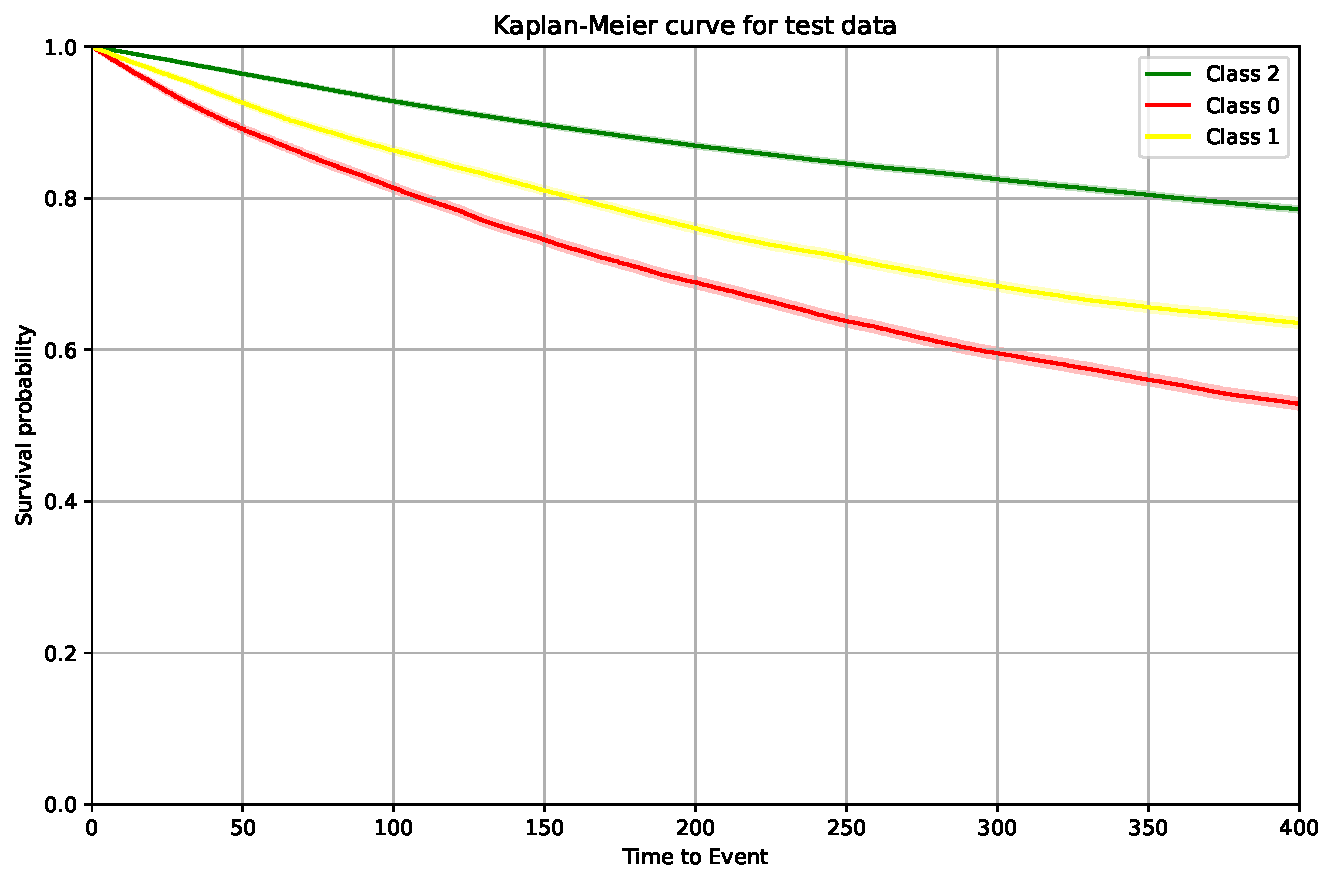
\includegraphics[width=\linewidth]{km_kNN_A.pdf}
%         \caption{kNN A}
%         \label{fig:km_knn_a}
%     \end{subfigure}
%     \hfill
%     \begin{subfigure}[t]{0.48\textwidth}
%         \centering
%         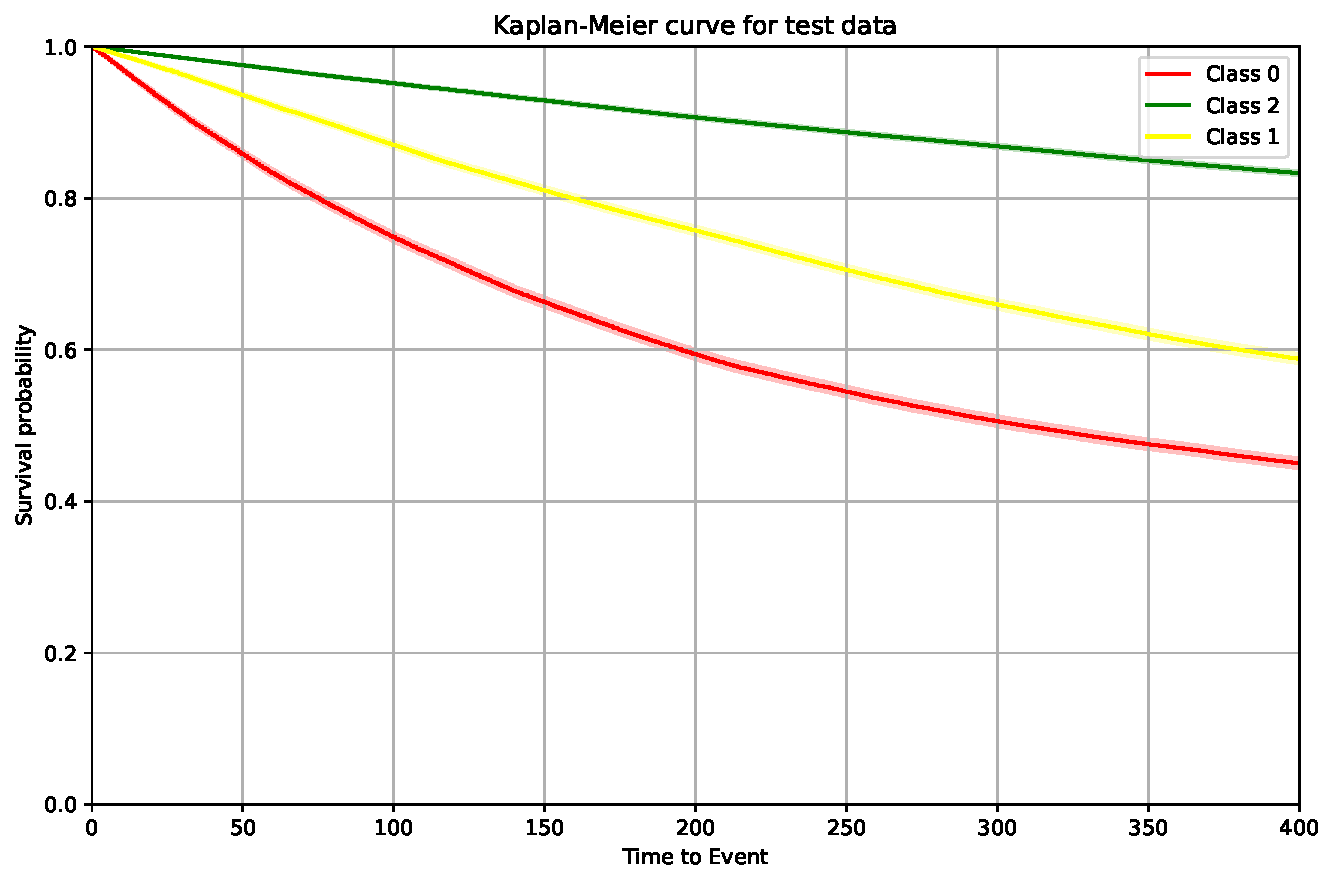
\includegraphics[width=\linewidth]{km_LSTM_A.pdf}
%         \caption{LSTM A}
%         \label{fig:km_lstm_a}
%     \end{subfigure}

%     \vspace{0.5cm}

%     \begin{subfigure}[t]{0.48\textwidth}
%         \centering
%         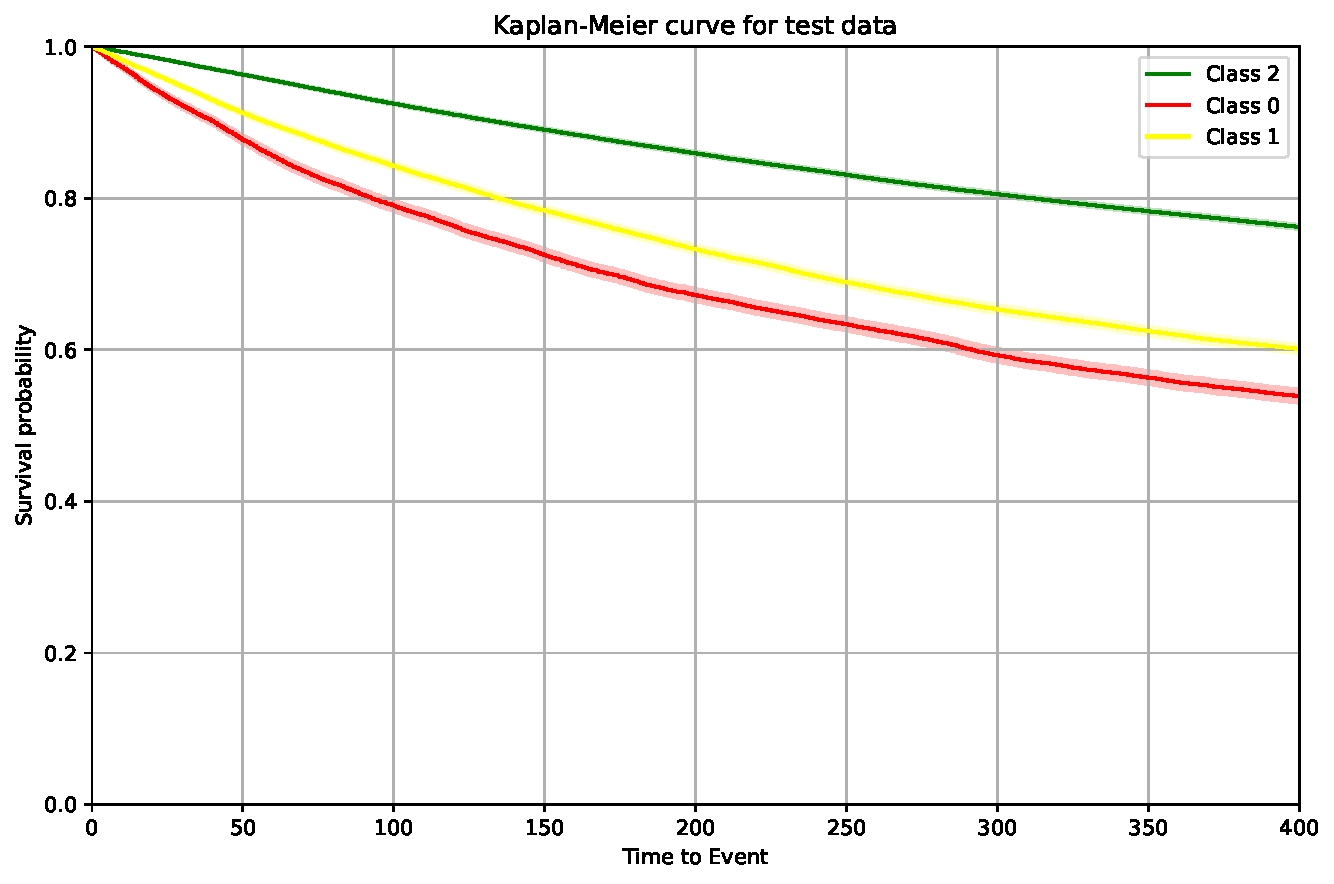
\includegraphics[width=\linewidth]{km_kNN_B.pdf}
%         \caption{kNN B}
%         \label{fig:km_knn_b}
%     \end{subfigure}
%     \hfill
%     \begin{subfigure}[t]{0.48\textwidth}
%         \centering
%         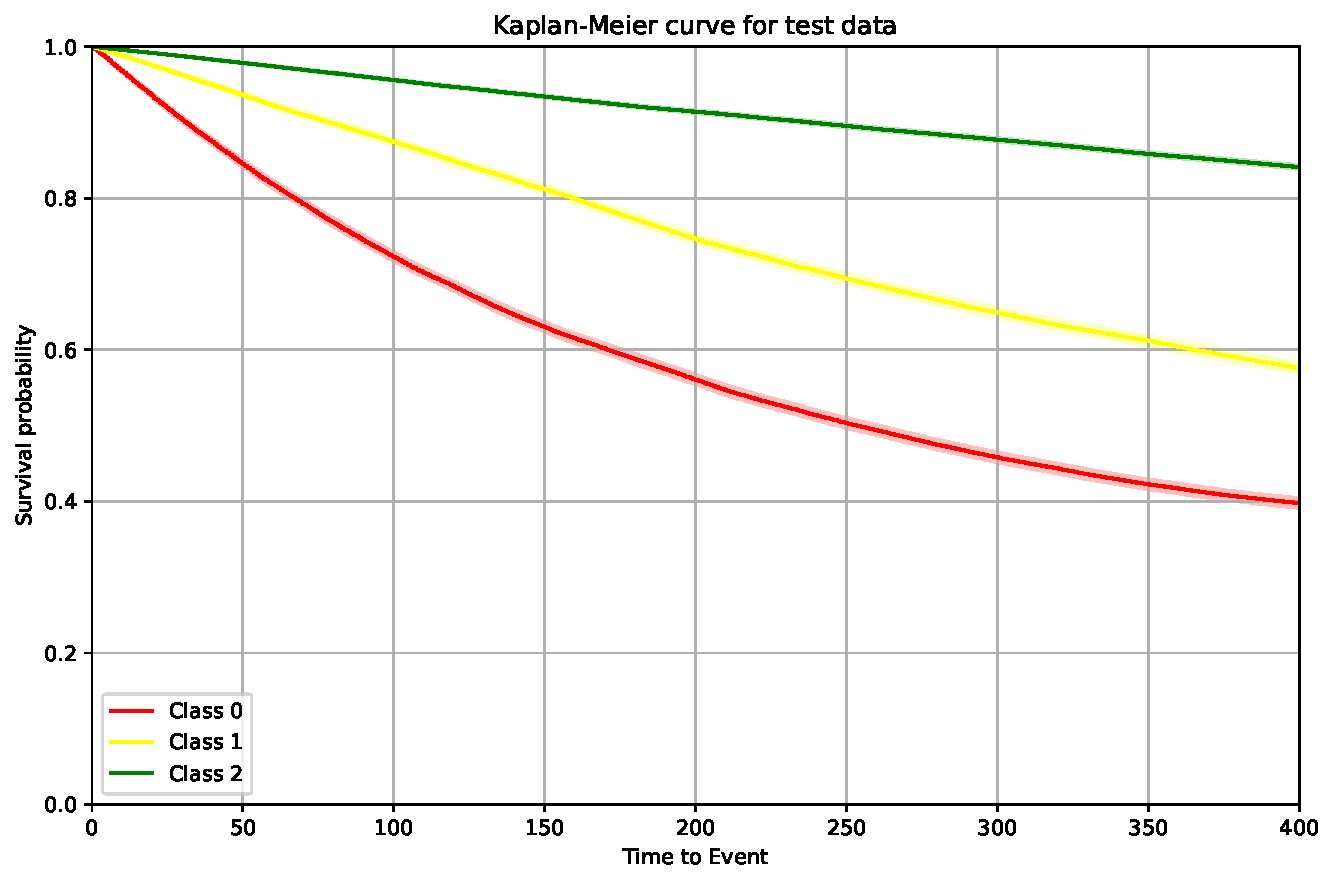
\includegraphics[width=\linewidth]{km_LSTM_B.pdf}
%         \caption{LSTM B}
%         \label{fig:km_lstm_b}
%     \end{subfigure}

%     \caption{Curve di Kaplan--Meier dei gruppi di rischio predetti
%     dai modelli kNN e LSTM sui dataset A e B.}
%     \label{fig:km_confronto}
% \end{figure}

% Confrontando le curve di Kaplan--Meier riportate nella Figura~\ref{fig:km_confronto}, in tutti e quattro i modelli le curve risultano ordinate coerentemente con i livelli di rischio previsti: il gruppo rosso (classe 0) presenta la sopravvivenza più bassa, il gruppo verde (classe 2) la più alta e il gruppo giallo (classe 1) una posizione intermedia, senza incroci nell'intervallo osservato. Il kNN A, addestrato sulla rappresentazione delle misurazioni mediante medie calcolate su finestre temporali, a 400 giorni mostra probabilità di sopravvivenza di circa 0,88 per la classe 2, 0,76 per la classe 1 e 0,69 per la classe 0. Il modello LSTM A raggiunge valori di circa 0,89, 0,75 e 0,71: il gruppo verde è leggermente più alto, ma le curve gialla e rossa risultano più ravvicinate (circa 0,04 a 400 giorni, contro circa 0,07 del kNN A), con una distanza minore lungo tutto l'intervallo. Per questa rappresentazione, quindi, LSTM A non presenta una separazione maggiore rispetto a kNN A: la distinzione tra la classe 2 e le altre due è simile nei due modelli, mentre quella tra la classe 1 e la classe 0 è meno marcata per LSTM A.

% Per quanto riguarda i modelli addestrati sulla rappresentazione basata sui parametri della regressione lineare calcolati sulle finestre temporali, il kNN B mostra una separazione sostanzialmente sovrapponibile a quella del kNN A; più nel dettaglio, a 400 giorni i valori sono di circa 0,87 per la classe 2, 0,74 per la classe 1 e 0,68 per la classe 0, e la distanza tra la curva verde e quella rossa (circa 0,19) è praticamente invariata rispetto a kNN A. Sulla base delle sole curve, quindi, non emergono evidenze che questa rappresentazione fornisca informazioni più utili alla stratificazione del rischio rispetto alla precedente.

% Infine, LSTM B presenta, sulla base dell'ispezione visiva, la separazione più ampia tra i gruppi: a 400 giorni le probabilità di sopravvivenza sono di circa 0,89 per la classe 2, 0,78 per la classe 1 e 0,69 per la classe 0, con distanze di circa 0,11 tra curva verde e gialla e 0,09 tra curva gialla e rossa. Le tre curve risultano inoltre distanziate in modo più regolare rispetto agli altri modelli, in cui la distanza tra curva gialla e rossa è compresa tra 0,04 e 0,07. La curva del gruppo rosso, tuttavia, non decresce più rapidamente di quella di kNN B (i valori finali sono quasi coincidenti, circa 0,69 e 0,68): il vantaggio di LSTM B deriva dalla posizione più alta delle curve gialla e verde. Nel complesso, LSTM B appare il modello più promettente tra quelli considerati per la stratificazione del rischio, ma le differenze rispetto agli altri modelli sono dell'ordine di 0,01--0,03 in probabilità di sopravvivenza e vanno interpretate con cautela.

\nocite{*}
\printbibliography

\end{document}